\documentclass[main.tex]{subfiles}
\title{Alex's lazy Sunday pancakes}

\begin{document}

\maketitle% this prints the handout title, author, and date

\begin{abstract}
Recipe makes 6 small bois or 2 thicc bois.  Serve with a tonne of Nutella, maple syrup, and maybe some ice cream for bonus husband points.
\end{abstract}

\section{Ingredients}

\vspace*{-\baselineskip}
\begin{table}[ht]
	\begin{tabularx}{\textwidth}{>{\hsize=0.333\hsize}X>{\bf\hsize=1\hsize}X}
	\unit[1]{cup} & all purpose flour\\
	\unit[1]{tsp} & sugar\\
	\unit[\nicefrac{1}{4}]{tsp} & ground cinnamon\\
	\unit[2]{tsp} & baking powder\\
	\unit[\nicefrac{1}{4}]{tsp} & salt\\
	\unit[1]{cup} & milk (I use soy milk but basically any should be fine)\\
	\unit[1]{tbsp} & vegetable oil\\
	\unit[1]{tbsp} & water \\
	\unit[1]{tsp} & vanilla extract\\
	\unit[2]{tbsp} & butter (melted)
	\end{tabularx}
\end{table}

\section{Instructions}

\begin{enumerate}
    \item Mix all of the ingredients together and whisk.
    \item Heat saucepan and add a little oil or butter.
    \item Add portions of pancake batter to the saucepan and cook for about 1 minute each side (maybe a little more or less depending on the heat).
    \item Enjoy!
\end{enumerate}

\begin{figure}
  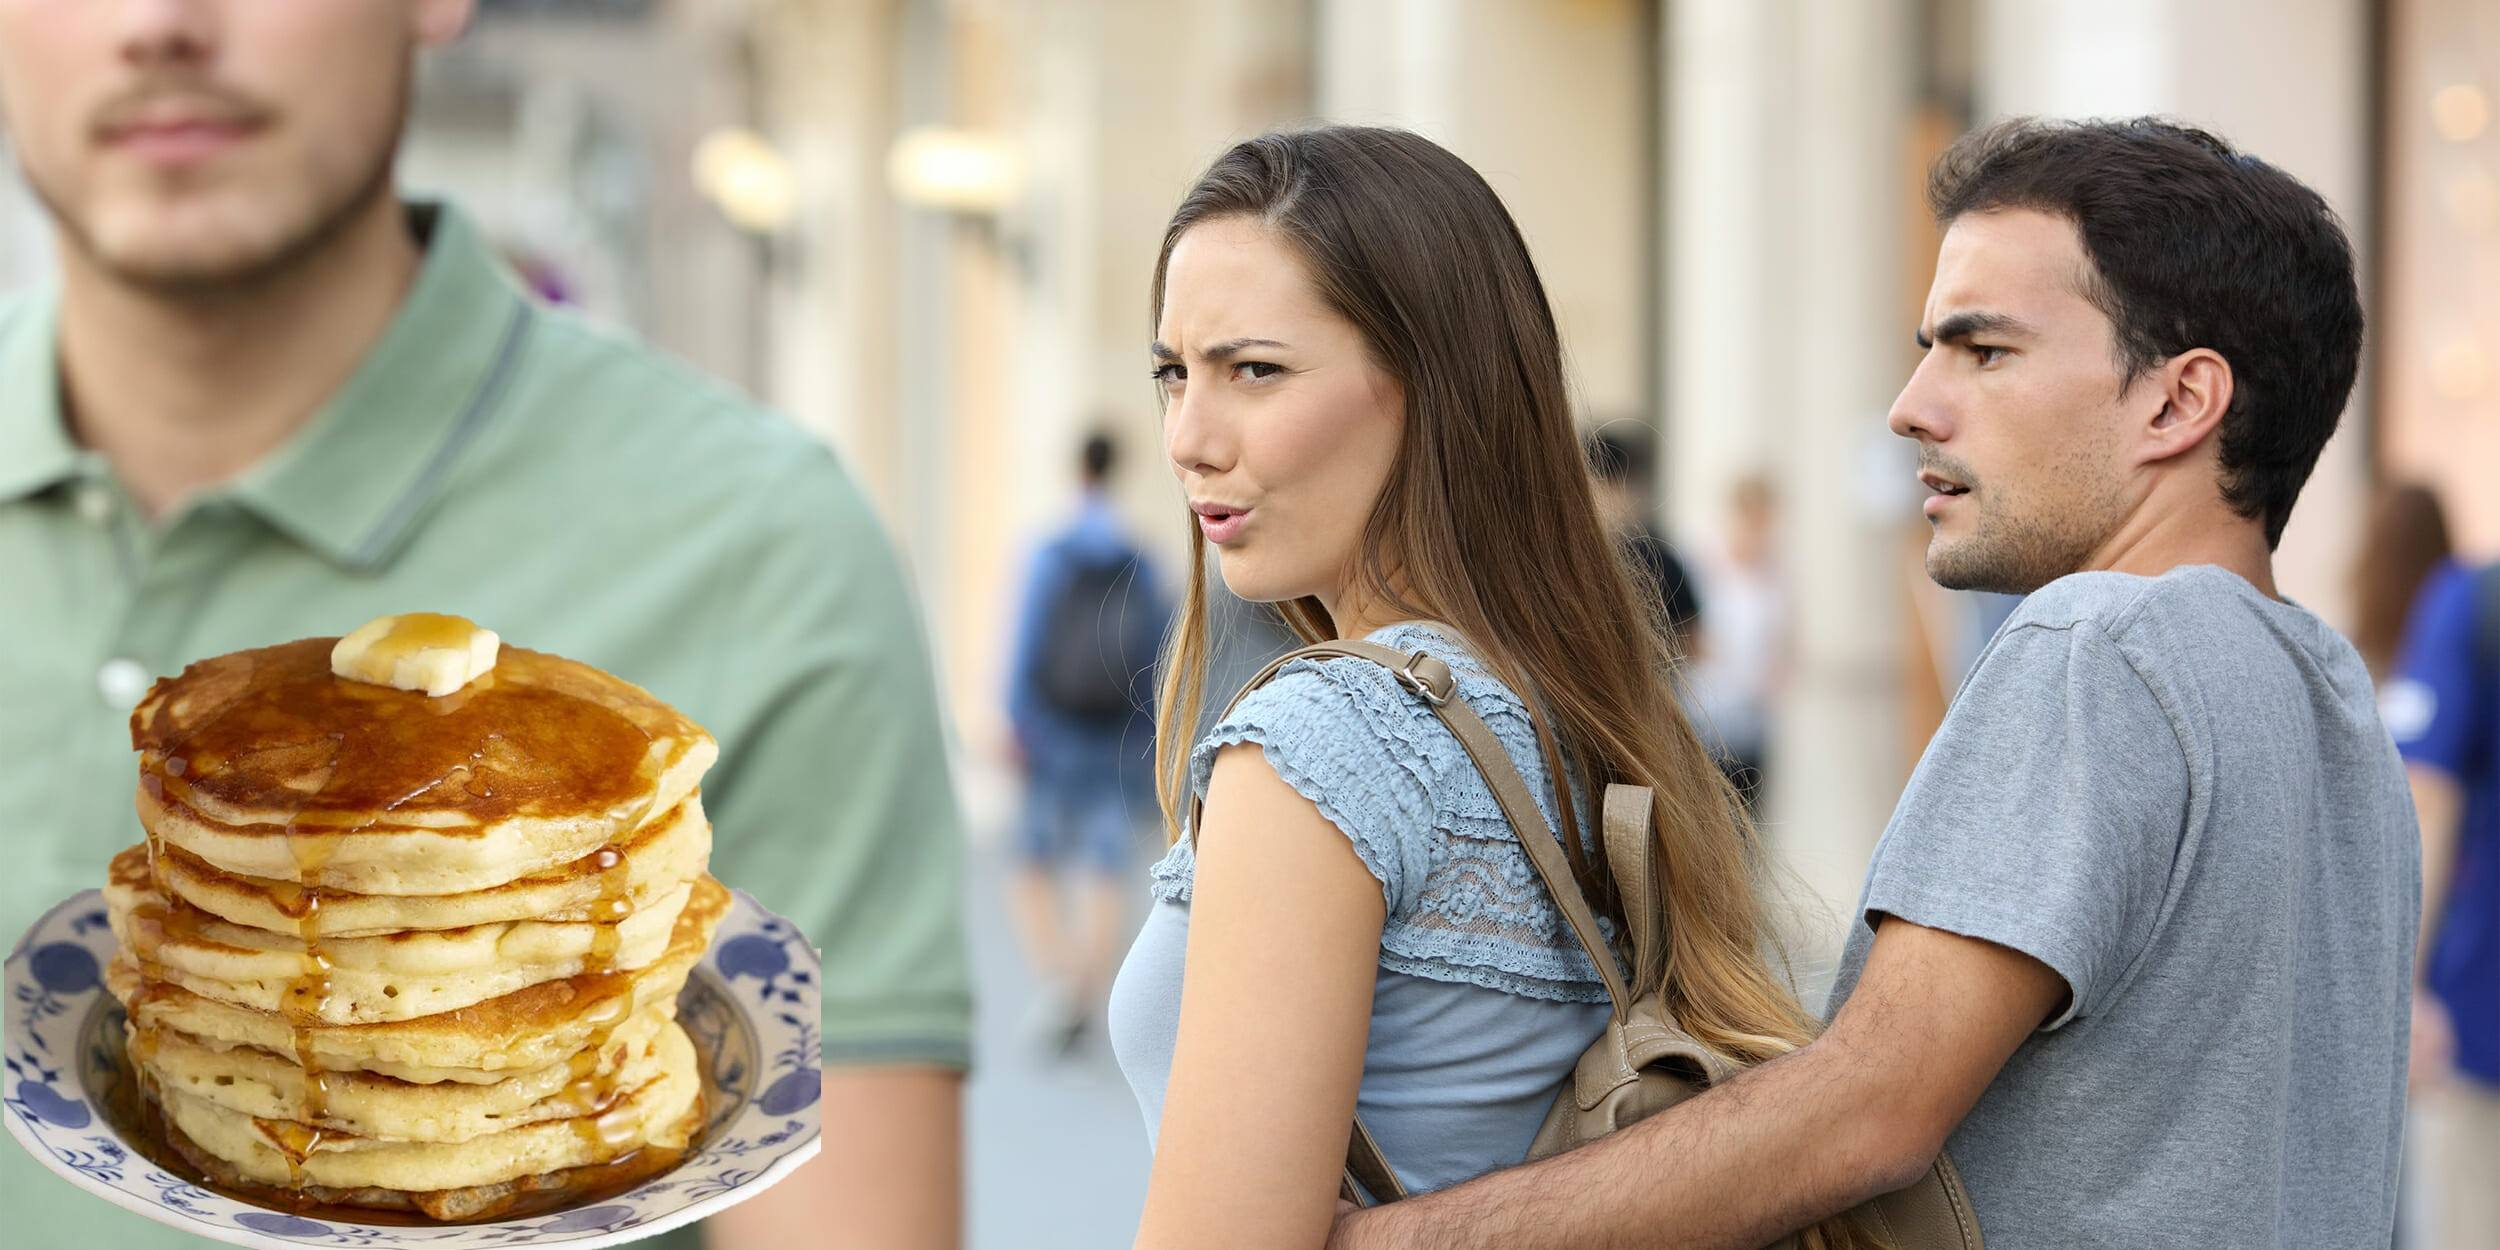
\includegraphics{alex-pancakes.jpg}
  \setfloatalignment{b}
\end{figure}
% \unit[325]{\textdegree F}

\end{document}
